\documentclass[12pt, a4paper]{article}
\usepackage[utf8]{inputenc}
\usepackage[T1]{fontenc}
\usepackage[magyar]{babel}
\usepackage{amsmath, amssymb}
\usepackage{xcolor}
\usepackage{tikz}
\usepackage{geometry}
\geometry{a4paper, margin=2.5cm}

% Új szín definiálása a megadott követelmények alapján
\definecolor{bvred}{rgb}{0.8, 0.0, 0.0}

% Új parancs a fontos részek kiemelésére
\newcommand{\textbfr}[1]{\textbf{\textcolor{bvred}{#1}}}

\begin{document}

\title{\textbfr{Kúpszeletek}}
\author{Készítette:\\Varga Dávid}
\date{}
\maketitle

\section*{Bevezetés a kúpszeletek elméletébe}

A geometria történetének egyik legszebb és leginkább vizuális témaköre a síkidomok térbeli származtatása. Amikor egy kettős kúpfelületet egy síkkal elmetszünk, a metszetként kapott görbéket összefoglaló néven kúpszeleteknek nevezzük. A metsző sík dőlésszögétől függően három fő, nem elfajuló esetet különböztetünk meg: a parabolát, az ellipszist (melynek speciális esete a kör) és a hiperbolát. 

Ezek a görbék nem csupán a tiszta matematikában játszanak kulcsszerepet, hanem a fizikában is: a bolygók pályája a Nap körül ellipszis, a ferdén elhajított test parabolapályán mozog, az alfa-részecskék pedig hiperbolapályán szóródnak az atommagokon.

\section*{1. A parabola}

A parabola a legegyszerűbb, egyetlen fókuszponttal rendelkező kúpszelet, amelyhez egy kitüntetett egyenes is tartozik.

\textbf{Definíció.} \textit{A sík azon pontjainak halmazát, amelyek egy adott egyenestől (vezéregyenes vagy direktrix) és egy rajta kívül fekvő adott ponttól (fókuszpont) egyenlő távolságra vannak, \textcolor{bvred}{parabolának} nevezzük.}

\subsection*{A parabola egyenletének levezetése}

Vegyünk fel egy derékszögű koordináta-rendszert úgy, hogy a parabola tengelypontja (csúcsa) az origóba essen, szimmetriatengelye pedig az $y$-tengely legyen. Legyen a fókuszpont távolsága az origótól $\frac{p}{2}$, ahol a $p$ paraméter a fókusz és a vezéregyenes távolsága. Ekkor a fókuszpont koordinátái $F\left(0, \frac{p}{2}\right)$, a vezéregyenes egyenlete pedig $y = -\frac{p}{2}$.

Legyen $P(x,y)$ a parabola egy tetszőleges pontja. A definíció értelmében a $P$ pont távolsága az $F$ ponttól megegyezik a vezéregyenestől mért távolságával ($d$). 
A két pont távolságára vonatkozó képlet alapján:
\[ \overline{PF} = \sqrt{x^2 + \left(y - \frac{p}{2}\right)^2} \]
A pont és a vízszintes vezéregyenes távolsága:
\[ d = \left| y - \left(-\frac{p}{2}\right) \right| = \left| y + \frac{p}{2} \right| \]
A definíció miatt a két távolság egyenlő:
\[ \sqrt{x^2 + \left(y - \frac{p}{2}\right)^2} = y + \frac{p}{2} \]
Mindkét oldalt négyzetre emelve (mivel a távolságok nem negatívak, az ekvivalencia megmarad):
\[ x^2 + y^2 - py + \frac{p^2}{4} = y^2 + py + \frac{p^2}{4} \]
Az azonos tagok egyszerűsítése és átrendezés után megkapjuk a parabola tengelyponti egyenletét:
\[ x^2 = 2py \]

Itt a $\textbfr{p}$ érték a parabola paramétere, amely meghatározza annak nyitottságát.

\subsection*{Geometriai reprezentáció}

Az alábbi ábrán egy felülről nyitott parabolát, annak fókuszpontját és vezéregyenesét láthatjuk. Figyeljük meg, hogy a $P$ pontból húzott két távolság egyenlő.

\begin{center}
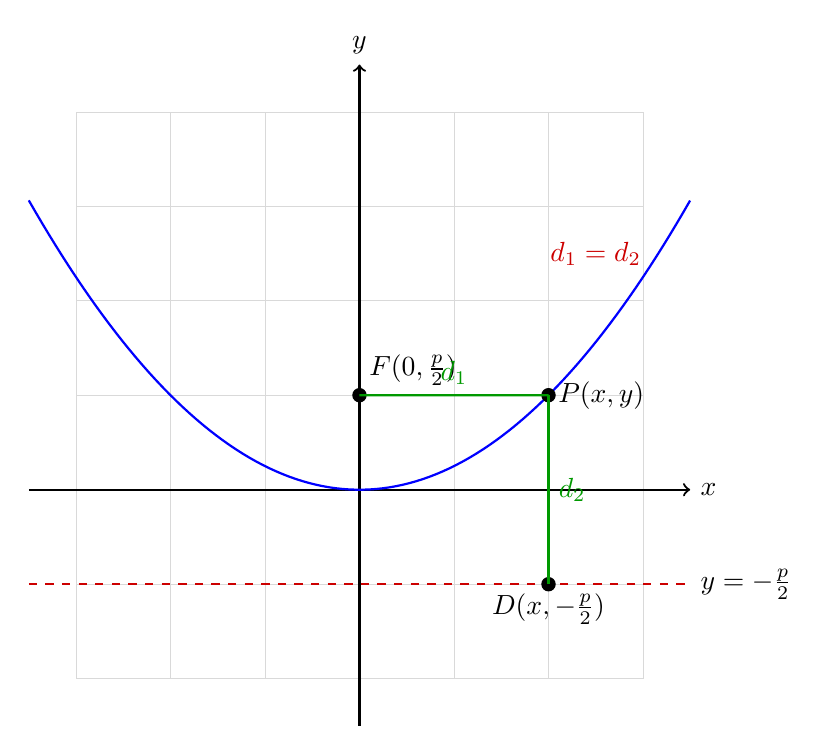
\begin{tikzpicture}[scale=1.2]
    % Rács és tengelyek
    \draw[step=1cm,gray!30,very thin] (-3,-2) grid (3,4);
    \draw[->,thick] (-3.5,0) -- (3.5,0) node[right] {$x$};
    \draw[->,thick] (0,-2.5) -- (0,4.5) node[above] {$y$};
    
    % Vezéregyenes (y = -1)
    \draw[bvred, thick, dashed] (-3.5,-1) -- (3.5,-1) node[right, text=black] {$y = -\frac{p}{2}$};
    
    % Parabola (x^2 = 4y -> y = x^2/4) p=2
    \draw[blue, thick, domain=-3.5:3.5, samples=100] plot (\x, {\x*\x/4});
    
    % Fókuszpont F(0, 1)
    \filldraw[black] (0,1) circle (2pt) node[above right] {$F(0, \frac{p}{2})$};
    
    % Tetszőleges P pont és távolságok
    \coordinate (P) at (2, 1);
    \coordinate (D) at (2, -1);
    \filldraw[black] (P) circle (2pt) node[right] {$P(x,y)$};
    \filldraw[black] (D) circle (2pt) node[below] {$D(x,-\frac{p}{2})$};
    
    \draw[thick, green!60!black] (P) -- (0,1) node[midway, above] {$d_1$};
    \draw[thick, green!60!black] (P) -- (D) node[midway, right] {$d_2$};
    
    \node at (2.5, 2.5) {\textbfr{$d_1 = d_2$}};
\end{tikzpicture}
\end{center}

\subsection*{Példák a parabola alkalmazására}
\begin{itemize}
    \item \textbf{Fényszórók:} A parabola forgatásával kapott forgási paraboloid belső felülete a fókuszpontba helyezett fényforrás sugarait párhuzamos nyalábban veri vissza.
    \item \textbf{Szabadon eső test:} Ha egy testet vízszintes sebességgel elhajítunk (légellenállás nélkül), pályájának egyenlete $y = -\frac{g}{2v_0^2}x^2$, ami egy lefelé nyitott parabola.
\end{itemize}

\section*{2. Az ellipszis}

Az ellipszis egy zárt görbe, amely leginkább egy "lapított körként" képzelhető el. A kör maga is az ellipszis egy speciális esete, amikor a két fókuszpont egybeesik.

\textbf{Definíció.} \textit{A sík azon pontjainak halmazát, amelyek két adott ponttól (fókuszpontok) mért távolságaik összege egy adott, a két fókuszpont távolságánál nagyobb állandó érték, \textcolor{bvred}{ellipszisnek} nevezzük.}

\subsection*{Az ellipszis egyenlete}

Legyen a két fókuszpont az $x$-tengelyen, az origóra szimmetrikusan: $F_1(-c, 0)$ és $F_2(c, 0)$. A fókusztávolság tehát $2c$. A definíció szerinti állandó távolságösszeget jelöljük $2a$-val (ahol $a > c > 0$).
Egy tetszőleges $P(x,y)$ pont pontosan akkor van az ellipszisen, ha:
\[ \overline{PF_1} + \overline{PF_2} = 2a \]
A távolságképleteket beírva:
\[ \sqrt{(x+c)^2 + y^2} + \sqrt{(x-c)^2 + y^2} = 2a \]
A kétszeres gyöktelenítés és algebrai átrendezés (amely meglehetősen hosszadalmas, de formális lépések sorozata) után bevezetjük a $b^2 = a^2 - c^2$ jelölést, mivel $a > c$ miatt $a^2 - c^2$ pozitív. Ebből a helyettesítésből az ellipszis középponti egyenlete:
\[ \frac{x^2}{a^2} + \frac{y^2}{b^2} = 1 \]

Ebben a képletben az $\textbfr{a}$ érték az ellipszis fél nagytengelye, a $\textbfr{b}$ érték pedig a fél kistengelye.

\begin{center}
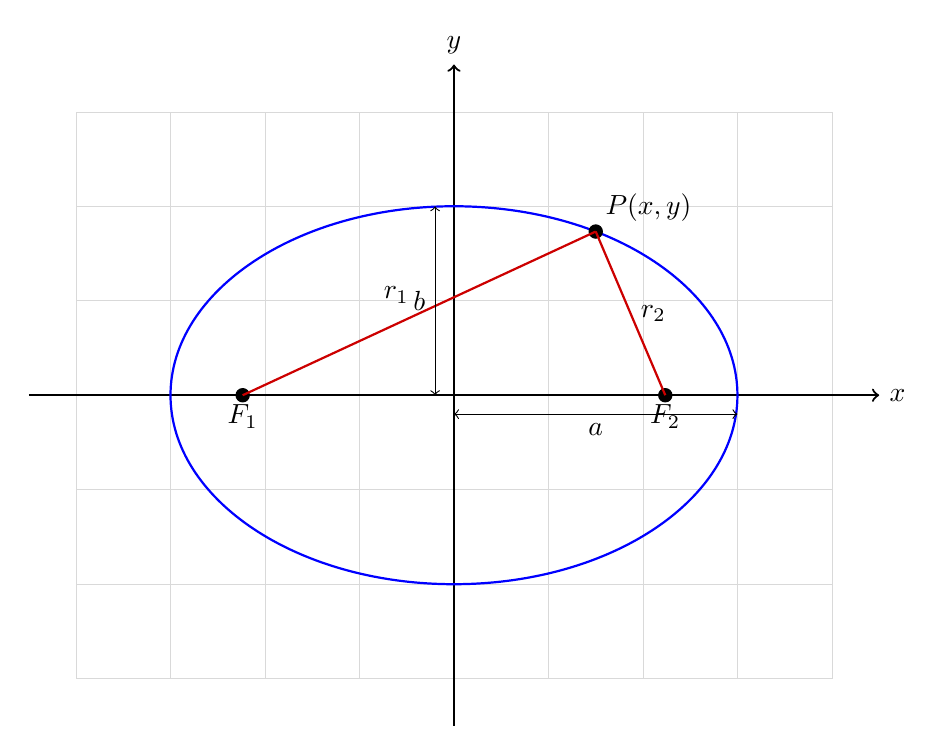
\begin{tikzpicture}[scale=1.2]
    % Rács és tengelyek
    \draw[step=1cm,gray!30,very thin] (-4,-3) grid (4,3);
    \draw[->,thick] (-4.5,0) -- (4.5,0) node[right] {$x$};
    \draw[->,thick] (0,-3.5) -- (0,3.5) node[above] {$y$};
    
    % Ellipszis (a=3, b=2)
    \draw[blue, thick] (0,0) ellipse (3 and 2);
    
    % Tengelyek és fókuszok (c = sqrt(3^2 - 2^2) = sqrt(5) ≈ 2.236)
    \coordinate (F1) at (-2.236, 0);
    \coordinate (F2) at (2.236, 0);
    \filldraw[black] (F1) circle (2pt) node[below] {$F_1$};
    \filldraw[black] (F2) circle (2pt) node[below] {$F_2$};
    
    % P pont
    \coordinate (P) at (1.5, 1.732);
    \filldraw[black] (P) circle (2pt) node[above right] {$P(x,y)$};
    
    % Vonalak P-ből a fókuszokba
    \draw[thick, bvred] (F1) -- (P) node[midway, above left, text=black] {$r_1$};
    \draw[thick, bvred] (P) -- (F2) node[midway, right, text=black] {$r_2$};
    
    % Feliratok az a és b megjelenítésére
    \draw[<->] (0,-0.2) -- (3,-0.2) node[midway, below] {$a$};
    \draw[<->] (-0.2,0) -- (-0.2,2) node[midway, left] {$b$};
\end{tikzpicture}
\end{center}

\subsection*{Példák az ellipszis alkalmazására}
\begin{itemize}
    \item \textbf{Kepler törvényei:} A Naprendszer bolygói olyan ellipszispályákon keringenek, amelyek egyik fókuszpontjában a Nap áll.
    \item \textbf{Orvosi alkalmazás (Liotripszia):} A vesekövek zúzására használt eszköz egy félellipszoid alakú kád. A hullámforrást az egyik fókuszba teszik, így a visszaverődő hullámok pontosan a másik fókuszban (a páciens vesekövénél) koncentrálódnak.
\end{itemize}

\end{document}